\documentclass[12pt,a4paper]{article}
\usepackage[utf8]{inputenc}
\usepackage[spanish,es-tabla]{babel}
\usepackage{amsmath}
\usepackage{amsfonts}
\usepackage{amssymb,latexsym,cancel}
\usepackage{graphicx}
\usepackage[left=2cm,right=2cm,top=2cm,bottom=2cm]{geometry}
\renewcommand{\baselinestretch}{1.5}
\usepackage{epstopdf}
\usepackage{subfigure}
\usepackage{array}
\usepackage{float}
\usepackage{longtable}
\newcolumntype{E}{>{$}c<{$}}
%%%%%%%%%%%%%%%%%%%%%%%%%%%
\usepackage{fancyhdr}
\pagestyle{fancy}
\fancyhead{}
\fancyhead[R]{ }
\fancyfoot[C]{\thepage}
\renewcommand{\headrulewidth}{0.9pt}
\renewcommand{\footrulewidth}{0.9pt}
\usepackage{url}


\begin{document}


\title{Actividad 4\\ Introducción a la biblioteca de visualización Matplotlib.  }
\author{
 Jorge Benz Olguín Aguilar\\
\small{División de Ciencias Exactas, Departamento de Física}\\
\small{Universidad de Sonora}\\
}
\date{\small{\today}}
\maketitle

\section*{Introducción}

\noindent Matplotlib es una biblioteca para la generación de gráficos a partir de datos contenidos en listas o arrays en el lenguaje de programación Python y su extensión matemática NumPy. Proporciona una API, pylab, diseñada para recordar a la de MATLAB.\cite{1}

\noindent También utilizamos NumPy, que es una extensión de Python, que le agrega mayor soporte para vectores y matrices, constituyendo una biblioteca de funciones matemáticas de alto nivel para operar con esos vectores o matrices. El ancestro de NumPy, Numeric, fue creado originalmente por Jim Hugunin con algunas contribuciones de otros desarrolladores. En 2005, Travis Oliphant creó NumPy incorporando características de Numarray en NumPy con algunas modificaciones. NumPy es open source. \cite{2}

\section*{Gráficas}


\noindent Para la práctica número cuatro utilizamos los datos que obtuvimos y analizamos en la Actividad 3; esto es, los datos de la estación Hermosillo del servicio meteorológico nacional. En primer lugar se nos pide elaborar una gráfica de barras (barplot) de precipitación mensual acumulada promedio de la colección de datos de la estación. Figura \ref{Fig:precipMenAcum}



\begin{figure}[H]
\centering
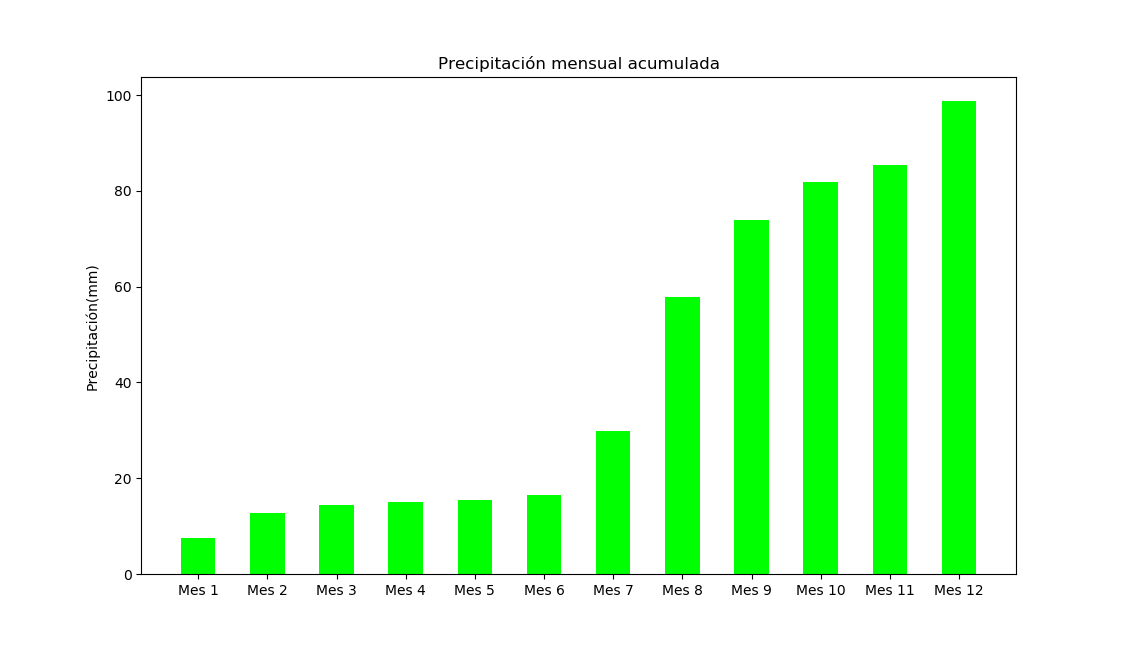
\includegraphics[scale=0.55]{PreciMesAcum.png}
\caption{}
\label{Fig:precipMenAcum}
\end{figure}

\noindent Podemos observar como a partir del mes 8 se da un drástico incremento en la precipitación acumulada, esto lo debemos a la temporada de lluvias que se da a a partir del 7 mes. 

\noindent En la gráfica que nos muestra la figura \ref{Fig:PrecipAnuaAcum} nos da la impresión de un aumento lineal de la precipitación acumulada, esto se debe a la carateristica de los datos que estamos graficando. Es mas facil visualizar  y analizar los datos, por mes, de la figura \ref{Fig:precipMenAcum}.


\begin{figure}[H]
\centering
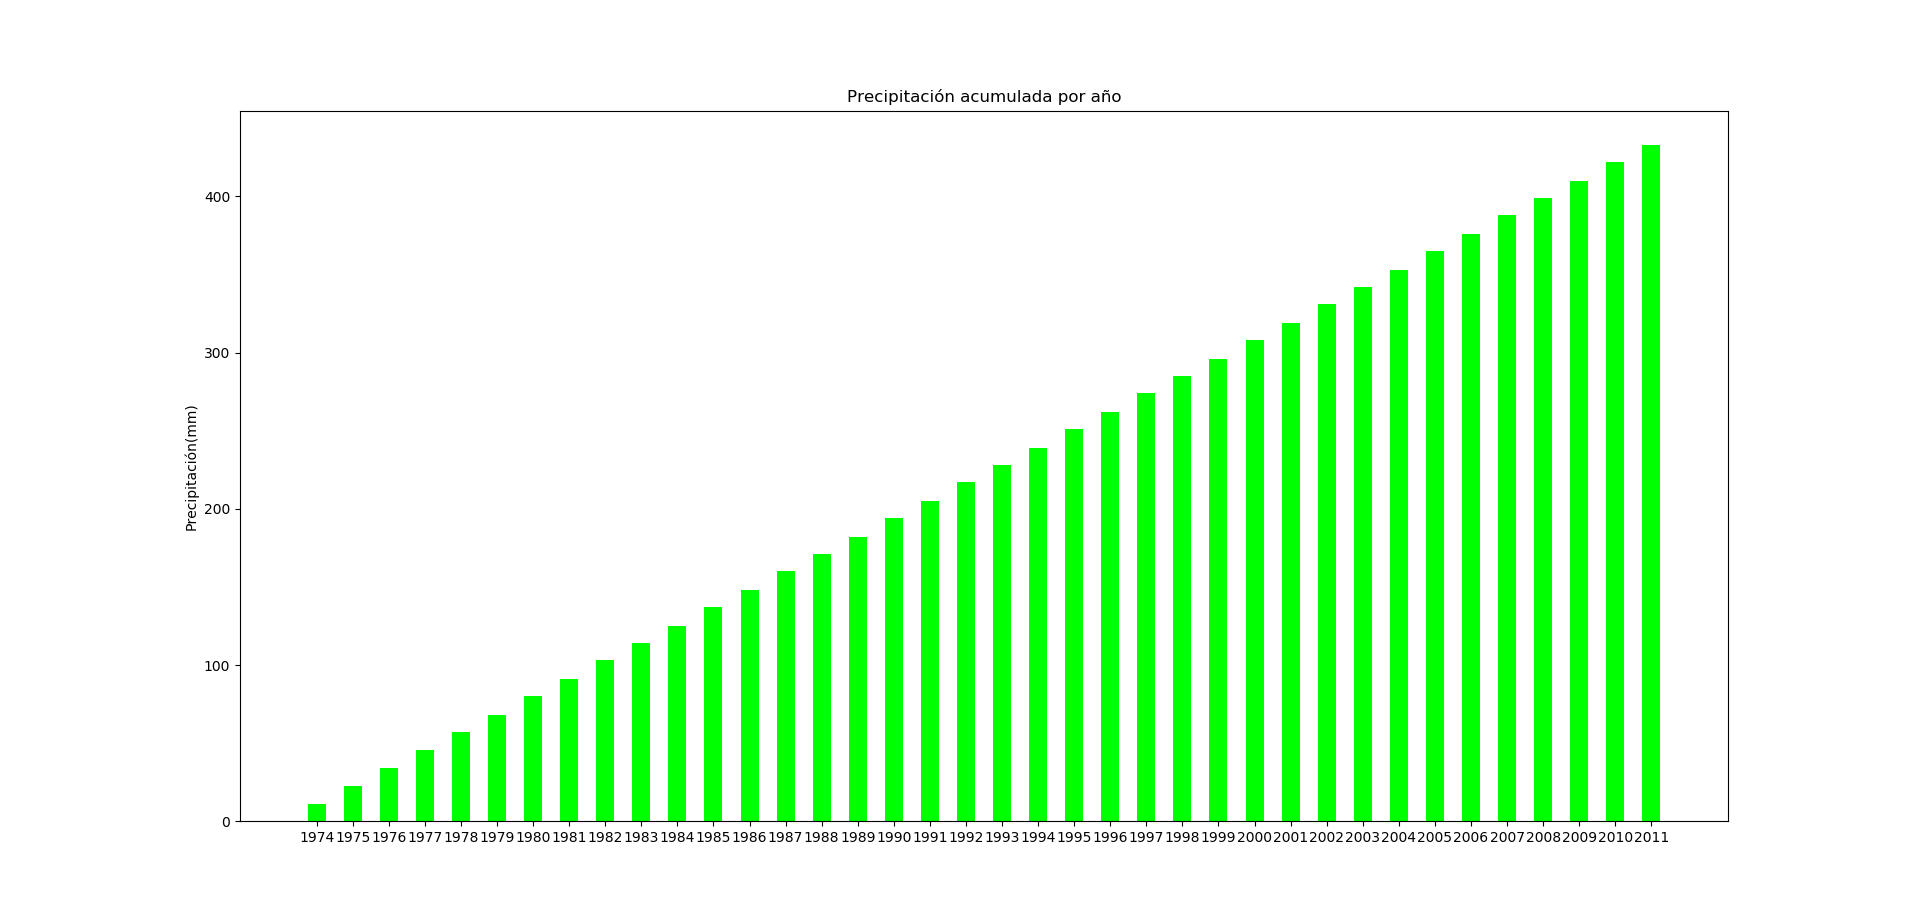
\includegraphics[scale=0.35]{PrecipAcum_ano.png}\caption{}
\label{Fig:PrecipAnuaAcum}
\end{figure}

La figura \ref{Fig:Tmaxminpmes} es la gráfica de dos curvas; la primera, temperaturas máximas de los meses del año y, la segunda temperaturas mínimas. El análisis de ellas es bastante claro; la curva naranja nos muestra como las temperaturas más altas se alcanzan en los meses de junio a septiembre; mientras que la curva azul, señala que en esos mismos meses obtenemos las mínimas más altas.  


\begin{figure}[H]
\centering
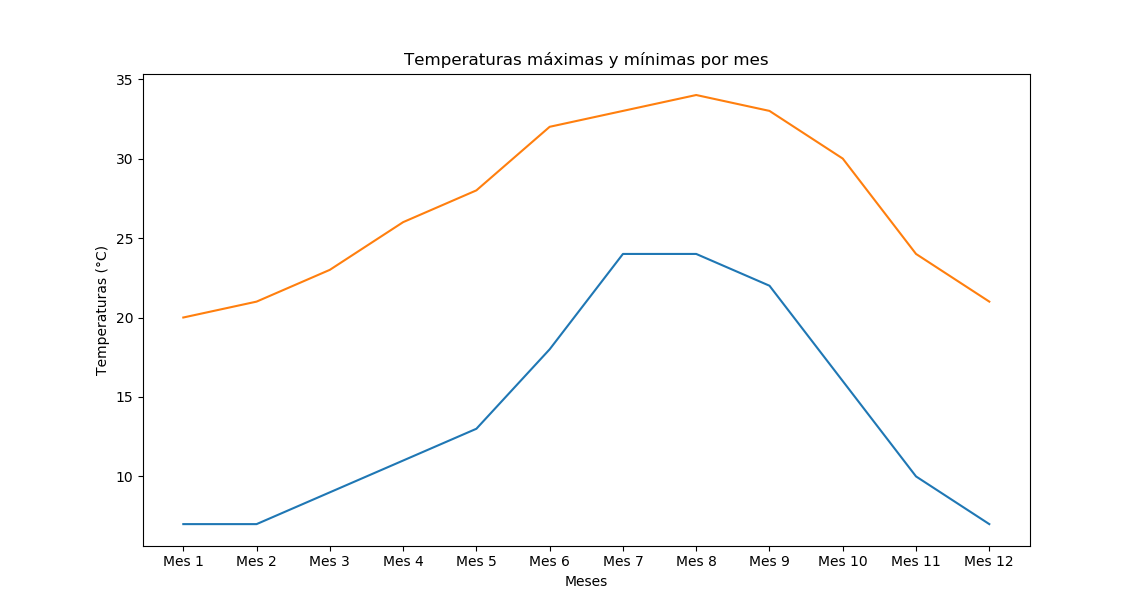
\includegraphics[scale=0.55]{Temp_max_min_mes.png} 
\caption{}
\label{Fig:Tmaxminpmes}
\end{figure}

\noindent El tipo de gráfica que utilizaremos y que podemos ver en la figura \ref{Fig:cajas1} es un método estandarizado para representar gráficamente una serie de datos numéricos a través de sus cuartiles, llamado boxplot. De esta manera, el diagrama de caja muestra a simple vista la mediana y los cuartiles de los datos, pudiendo también representar los valores atípicos de estos. 

\noindent La gráfica de la izquierda nos muestra una acumulación de los datos entre 8 y 18 grados centígrados, y podemos ver a la mediana rondando los  $12.5 ^{\circ} $C

\begin{figure}[H]
\centering
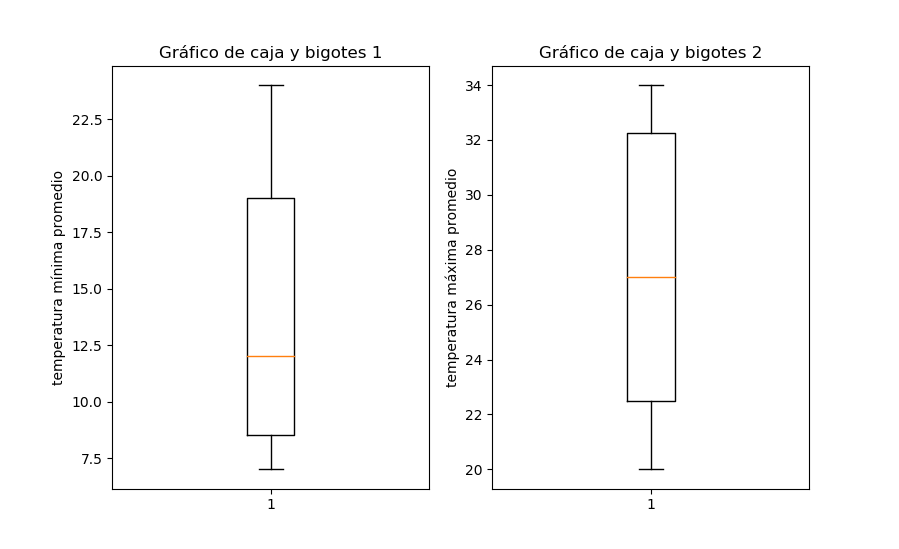
\includegraphics[scale=0.45]{Temp_pro_mensual_cajas.png} 
\caption{}
\label{Fig:cajas1}
\end{figure}

Ahora bien, en la gráfica de la derecha, nos muestra que la distribución de los datos se encuentra entre aproximadamente 23 y 32 grados centígrados, con una media por los $27 ^{\circ}$C.

\noindent En la figura \ref{Fig:cajas2} podemos observar una gran concentración de los datos y esto gracias a que a simple vista podemos una caja muy pequeña en comparación con la distribución de los datos, de hecho los círculos nos muestran algunos datos atípicos que no se suelen tomar en cuenta.



\begin{figure}[H]
\centering
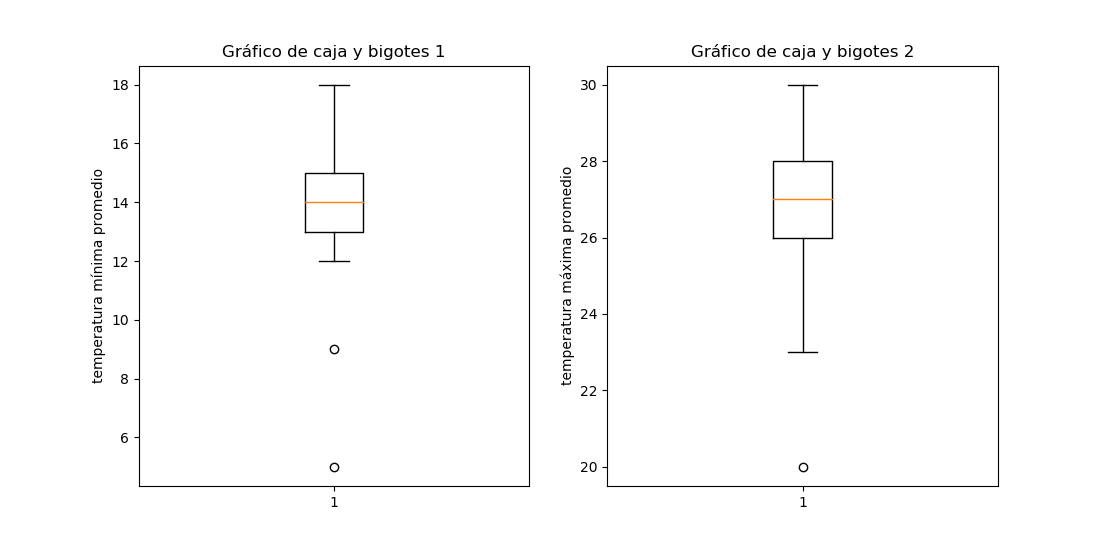
\includegraphics[scale=0.45]{Cajas_bigotes_temp_anual.png} 
\caption{}
\label{Fig:cajas2}
\end{figure}


\noindent Es importante notar lo poderosa que son las gráficas para interpretar una colección de datos. Las herramientas técnicas como la biblioteca de matplotlib; la extensión numpy y, la biblioteca pandas, para el manejo de los datos, nos permiten manipularlos y graficarlos para poder analizarlos.
 



\begin{thebibliography}{0}


\bibitem {1}Matplotlib. (2017, 11 de noviembre). Wikipedia, La enciclopedia libre. Fecha de consulta: 03:37, febrero 24, 2019 

\bibitem {2}NumPy. (2018, 4 de octubre). Wikipedia, La enciclopedia libre. Fecha de consulta: 04:01, febrero 27, 2019 


\end{thebibliography}

\end{document}

